\chapter{Resultados}
 \label{cap5_resultados}

\section{Resultados da Simulação Computacional}

Com o objetivo de avaliar o comportamento do sistema fotovoltaico automatizado, foi realizada uma simulação computacional utilizando o ambiente MATLAB/Simulink. O modelo desenvolvido permitiu comparar o desempenho de um sistema automatizado, capaz de manter o painel orientado em direção à maior incidência da radiação solar, com um sistema fotovoltaico de painel fixo.

A simulação foi executada para um período correspondente a 12 horas de operação, representando o intervalo aproximado entre o nascer e o pôr do Sol, utilizando as condições descritas na metodologia. A Figura~\ref{fig:potencia_simulacao} apresenta as curvas de potência obtidas para os sistemas automatizado e de painel fixo durante o período de simulação.

\begin{figure}[H]
\centering
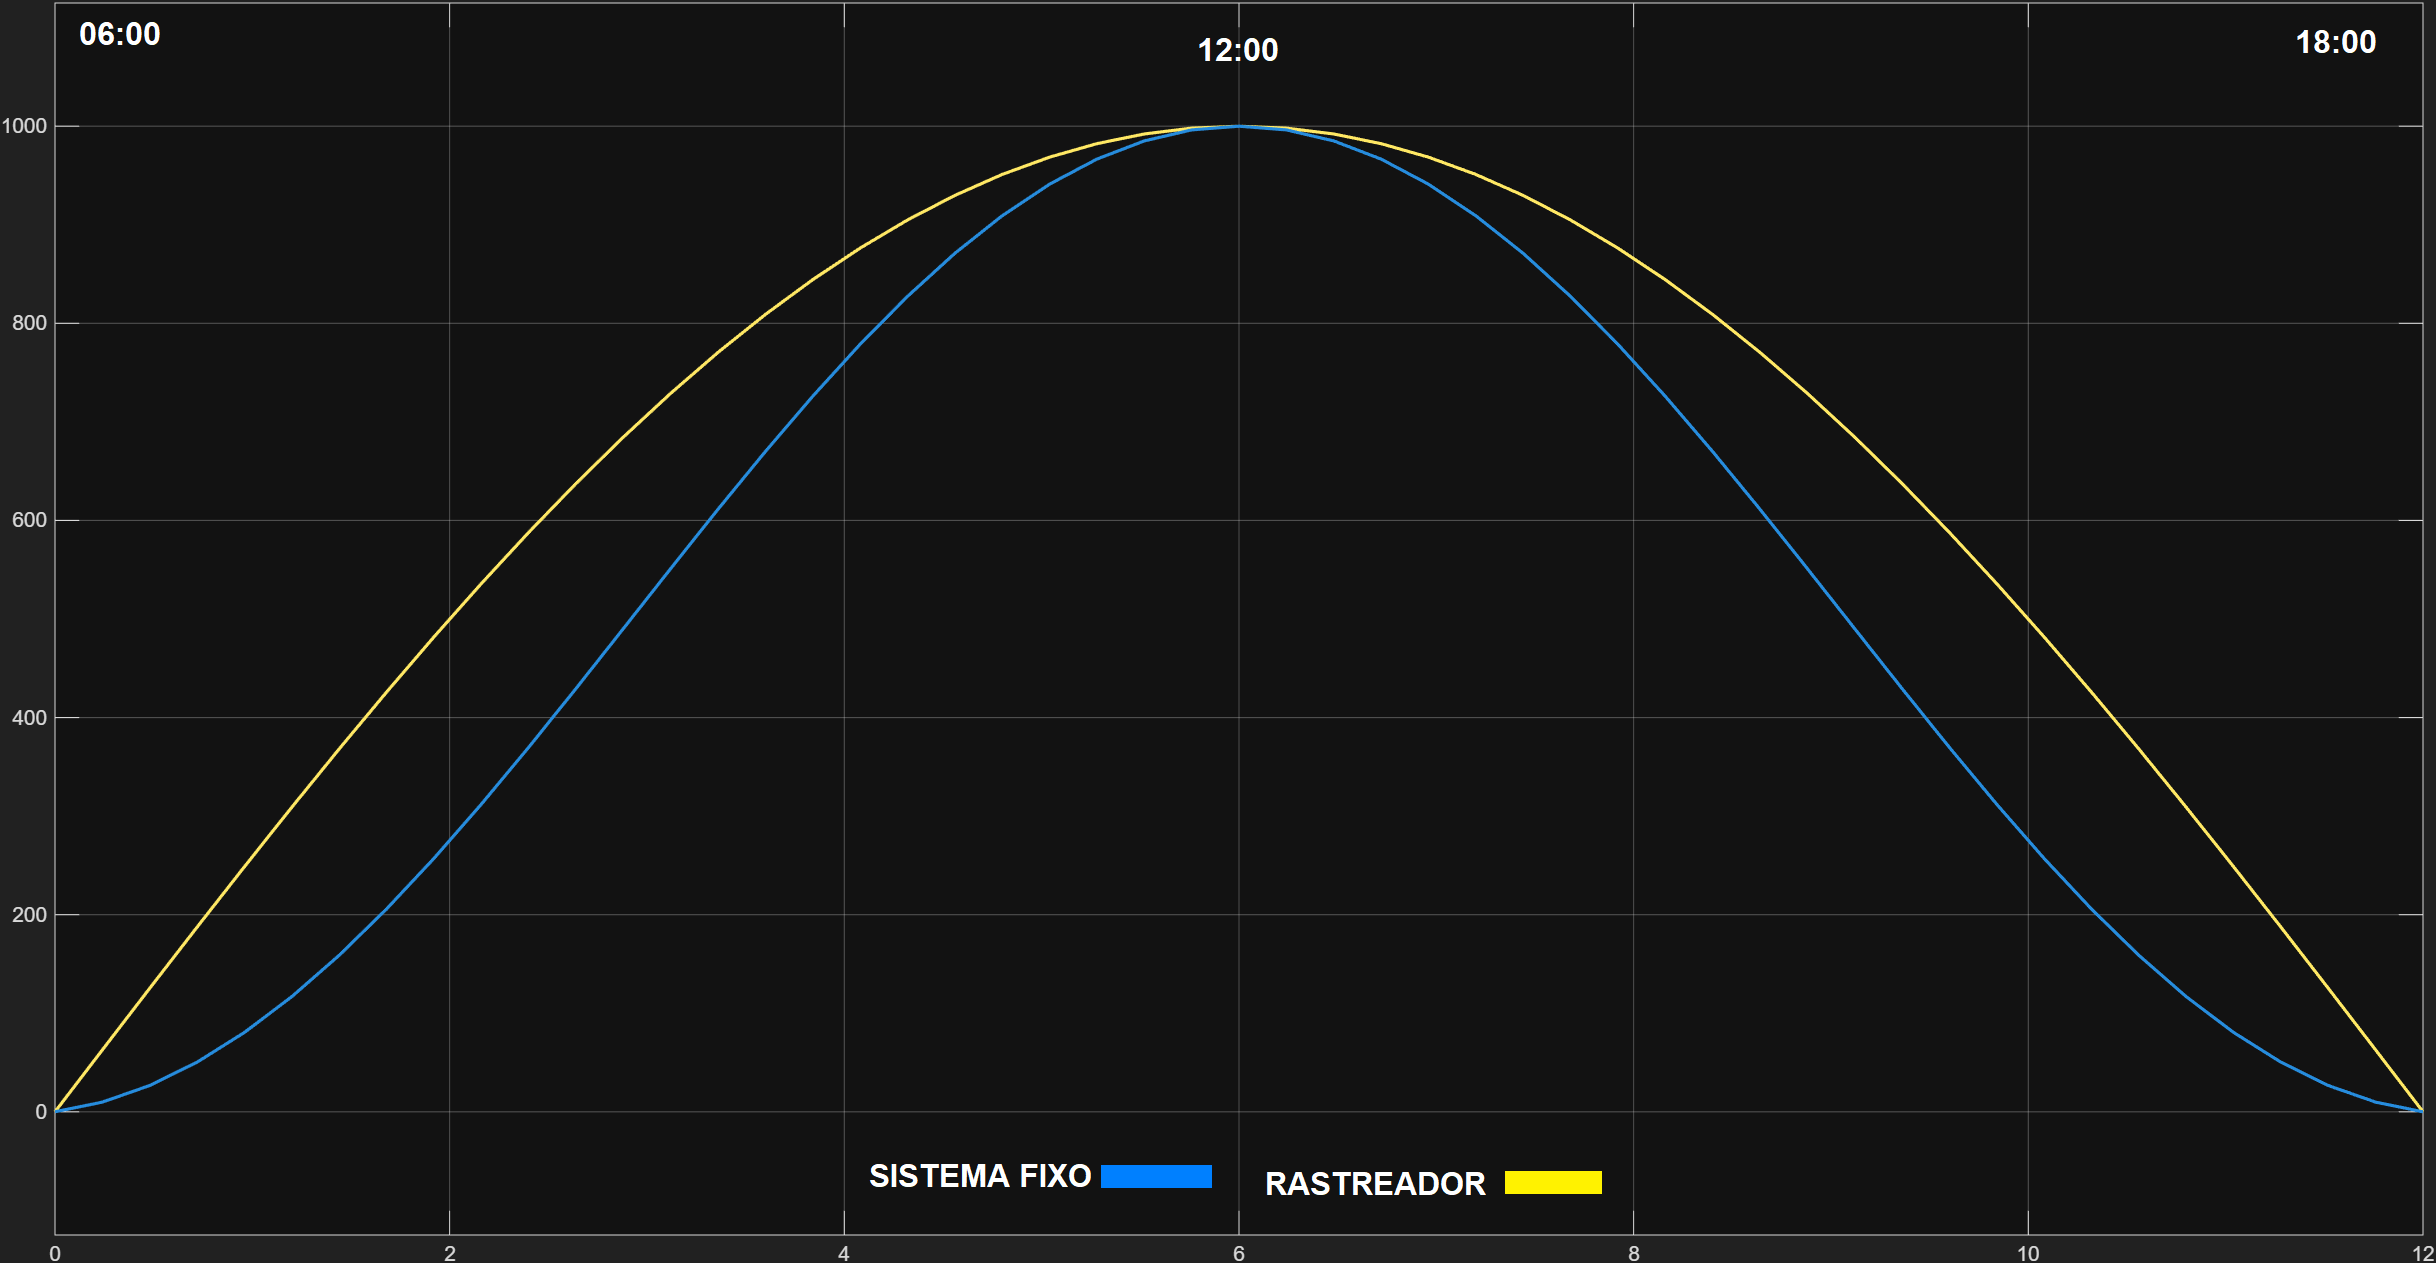
\includegraphics[width=0.85\textwidth]{Figuras/grafico_MS.png}
\caption{Curvas de potência obtidas na simulação computacional.}
\label{fig:potencia_simulacao}
\fonte{Autor (2026).}
\end{figure}

Observa-se que ambas as curvas acompanham a variação da irradiância ao longo do dia, apresentando aumento gradual da potência durante o período da manhã, valor máximo próximo ao meio-dia e redução ao longo da tarde. Entretanto, durante praticamente todo o período de simulação, o sistema automatizado apresentou valores de potência superiores aos do sistema de painel fixo.

Esse comportamento ocorre porque o modelo considera que o painel automatizado permanece continuamente orientado na direção de maior incidência da radiação solar, enquanto o painel fixo sofre perdas decorrentes da variação do ângulo de incidência da radiação ao longo do dia.

A integração das curvas de potência permitiu determinar a energia acumulada produzida por cada sistema durante todo o período de simulação. A partir desses valores foi calculado o ganho energético percentual do sistema automatizado em relação ao sistema de painel fixo.

Os resultados indicaram um ganho energético de aproximadamente \textbf{23,94\%}, evidenciando que o reposicionamento automatizado do painel proporciona maior aproveitamento da irradiância incidente e, consequentemente, maior geração de energia quando comparado ao sistema com painel fixo.

Embora o modelo utilize simplificações em relação às condições reais de operação, como irradiância idealizada e ausência de efeitos atmosféricos, os resultados obtidos apresentaram comportamento compatível com o esperado para sistemas fotovoltaicos com rastreamento solar de eixo único, fornecendo uma referência para a comparação com os dados experimentais obtidos pelo protótipo físico.

Na seção seguinte, os resultados da simulação são comparados aos dados experimentais, permitindo avaliar a capacidade do modelo computacional em representar o comportamento observado no sistema desenvolvido.

\section{Desempenho Experimental do Sistema}

Esta seção apresenta os resultados obtidos durante os ensaios experimentais realizados com o sistema fotovoltaico automatizado e com o sistema fotovoltaico de painel fixo. Conforme descrito na metodologia, ambos os sistemas operaram simultaneamente sob as mesmas condições ambientais, possibilitando a comparação direta de seus desempenhos ao longo do período experimental.

Os ensaios foram realizados entre os dias 23 e 26 de maio de 2026, com aquisição automática das variáveis elétricas entre 06h00 e 18h00, em intervalos de um minuto. A potência elétrica instantânea foi calculada a partir das medições de tensão e corrente registradas pelo sistema, conforme a Equação~\ref{eq:potencia}.

A energia produzida por cada sistema foi obtida pela integração numérica da potência ao longo do período de operação, permitindo determinar a produção energética diária de cada configuração. Com base nesses resultados, foi calculado o ganho percentual proporcionado pelo sistema automatizado em relação ao sistema de painel fixo.

Os resultados experimentais são apresentados inicialmente por meio das curvas de potência instantânea obtidas em cada dia de coleta. Em seguida, são analisados os valores de energia acumulada e o ganho energético proporcionado pelo sistema automatizado em comparação ao sistema de painel fixo. Por fim, os resultados experimentais são comparados aos obtidos pelo modelo computacional desenvolvido no MATLAB/Simulink, permitindo avaliar a representatividade da simulação em relação ao comportamento observado no protótipo físico.

\subsection{Curvas de Potência Instantânea}

As Figuras~\ref{fig:pot23}, \ref{fig:pot24}, \ref{fig:pot25} e~\ref{fig:pot26} apresentam as curvas de potência elétrica instantânea obtidas para o sistema automatizado e para o sistema com painel fixo durante os quatro dias de coleta experimental.

\begin{figure}[H]
\centering
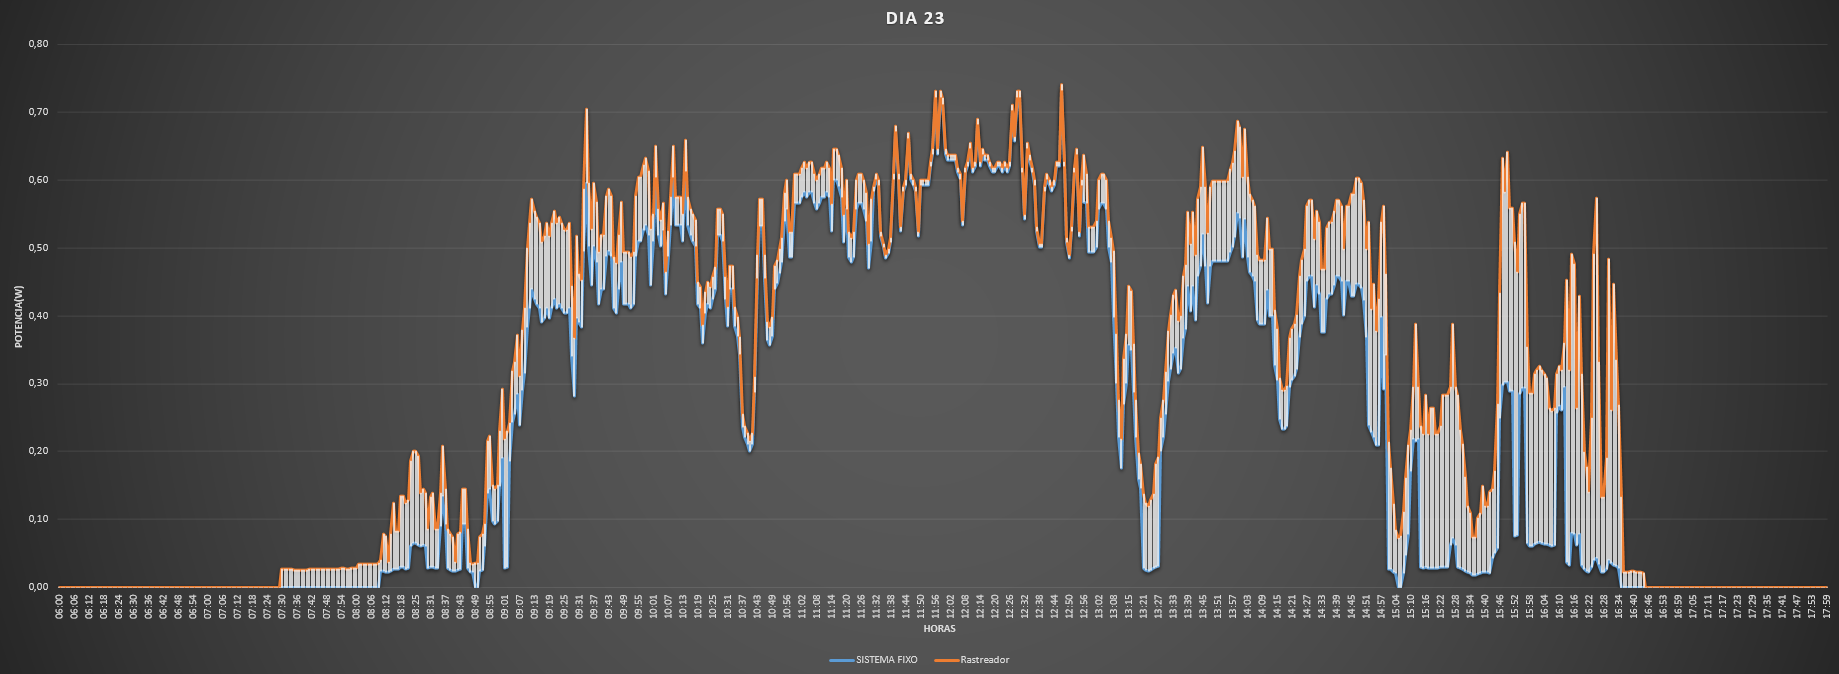
\includegraphics[width=0.90\textwidth]{Figuras/23_POTENCIA.png}
\caption{Curvas de potência dos sistemas automatizado e fixo em 23/05/2026.}
\label{fig:pot23}
\fonte{Autor (2026).}
\end{figure}

\begin{figure}[H]
\centering
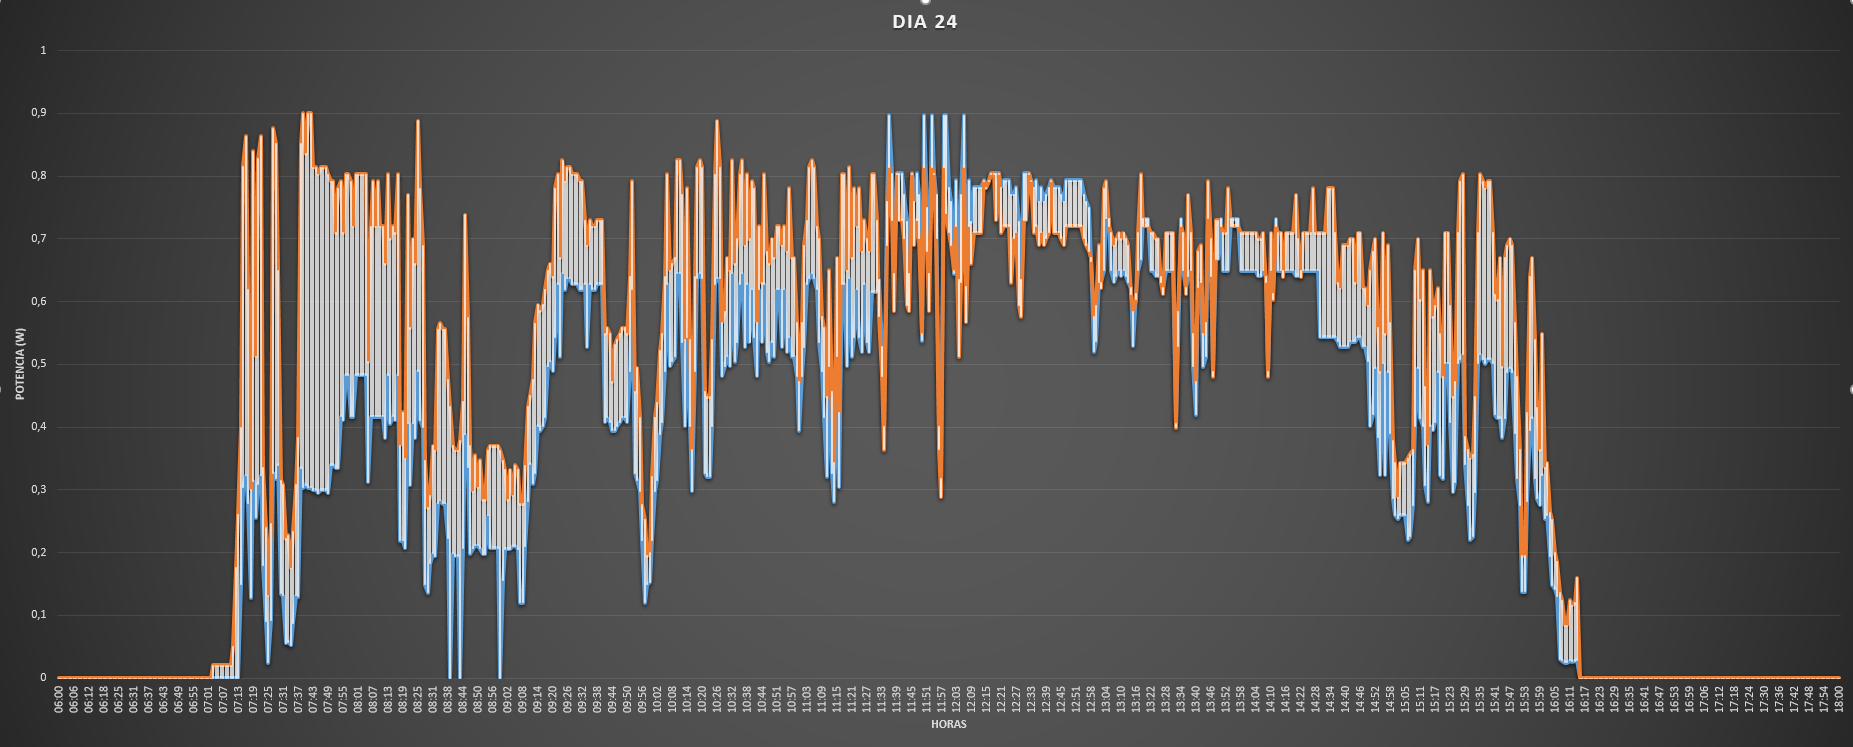
\includegraphics[width=0.90\textwidth]{Figuras/24_POTENCIA.png}
\caption{Curvas de potência dos sistemas automatizado e fixo em 24/05/2026.}
\label{fig:pot24}
\fonte{Autor (2026).}
\end{figure}

\begin{figure}[H]
\centering
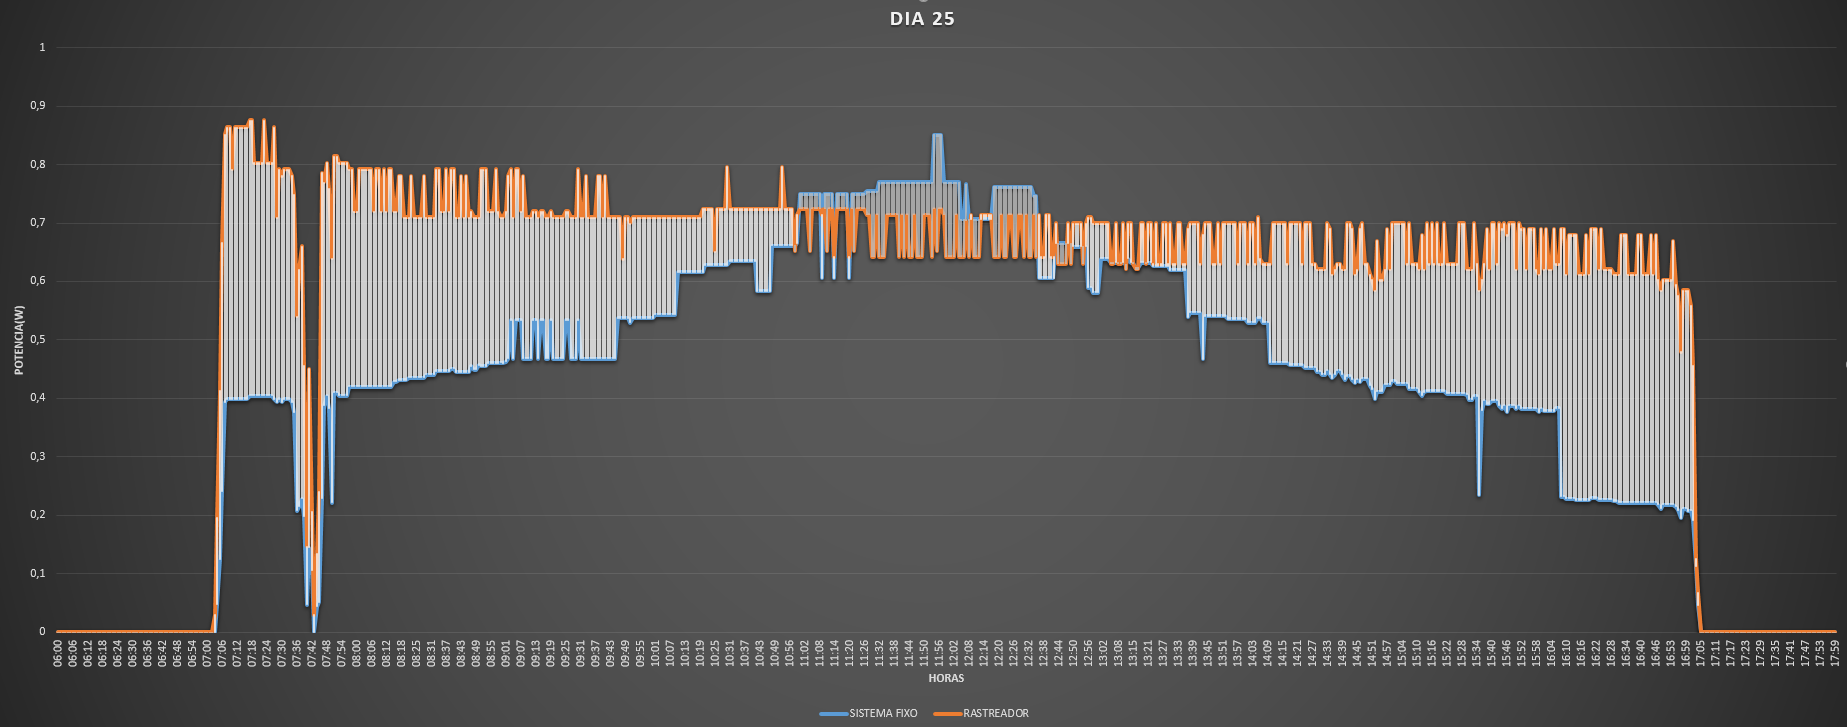
\includegraphics[width=0.90\textwidth]{Figuras/25_POTENCIA.png}
\caption{Curvas de potência dos sistemas automatizado e fixo em 25/05/2026.}
\label{fig:pot25}
\fonte{Autor (2026).}
\end{figure}

\begin{figure}[H]
\centering
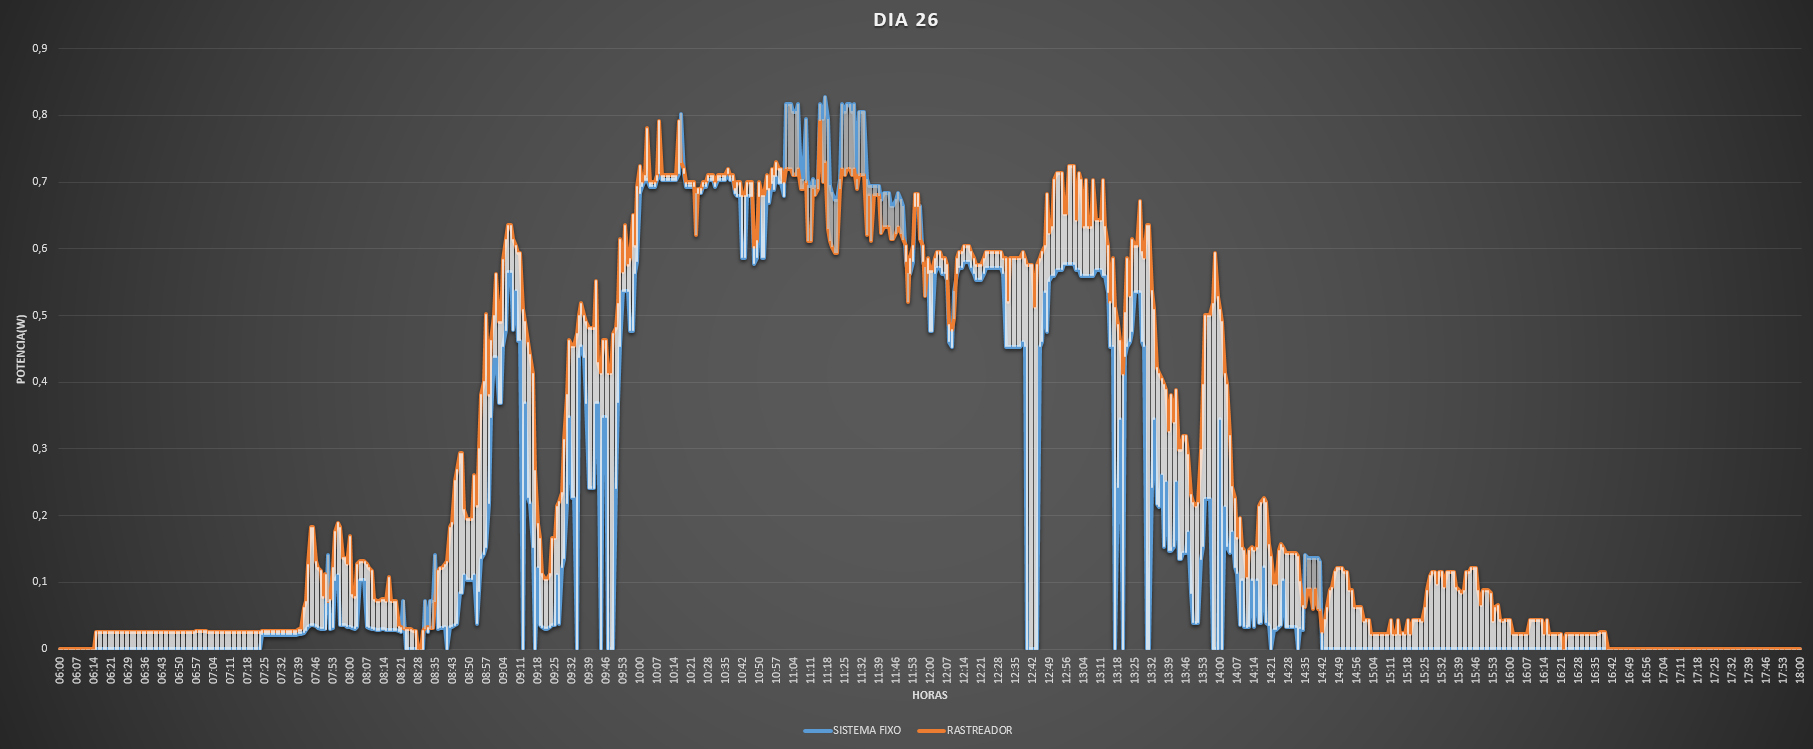
\includegraphics[width=0.90\textwidth]{Figuras/26_POTENCIA.png}
\caption{Curvas de potência dos sistemas automatizado e fixo em 26/05/2026.}
\label{fig:pot26}
\fonte{Autor (2026).}
\end{figure}

A análise conjunta das Figuras~\ref{fig:pot23} a~\ref{fig:pot26} evidencia um comportamento semelhante entre os quatro dias de ensaio. Em ambos os sistemas, a potência aumenta gradativamente após o nascer do Sol, atinge valores máximos próximos ao período de maior incidência da radiação solar e diminui progressivamente ao longo da tarde até o pôr do Sol.

Observa-se que o sistema automatizado apresentou valores de potência superiores aos do sistema com painel fixo durante a maior parte do período de operação. Esse comportamento está diretamente relacionado ao ajuste contínuo da orientação do painel fotovoltaico, reduzindo o ângulo de incidência da radiação solar sobre a superfície do módulo e aumentando o aproveitamento da irradiância disponível.

Embora ambos os sistemas tenham sido submetidos às mesmas condições ambientais, pequenas oscilações podem ser observadas nas curvas de potência ao longo do dia. Essas variações estão associadas principalmente à passagem de nuvens, alterações temporárias na irradiância solar, variações na temperatura das células fotovoltaicas e às incertezas inerentes ao processo de medição dos sensores utilizados.

Além dessas variações, observa-se que o sistema automatizado apresenta pequenas oscilações adicionais decorrentes da estratégia de controle implementada no algoritmo. Em intervalos regulares, o sistema realiza uma rotina de otimização local, efetuando pequenos deslocamentos angulares em torno da posição de referência e comparando a potência elétrica obtida em cada posição. Após essa comparação, o painel é reposicionado automaticamente no ângulo que proporciona a maior potência instantânea, o que resulta em pequenas variações nas curvas registradas.

Outro aspecto observado é que o ganho proporcionado pelo sistema automatizado torna-se mais evidente durante os períodos da manhã e da tarde. Nesses horários, o sistema com painel fixo apresenta maiores perdas decorrentes do aumento do ângulo de incidência da radiação solar, enquanto o sistema automatizado mantém o painel orientado de forma mais favorável. Próximo ao meio-dia, quando ambos os sistemas apresentam orientação semelhante em relação ao Sol, a diferença entre as potências tende a diminuir.

De maneira geral, os resultados experimentais demonstram que a estratégia de posicionamento adotada permitiu aumentar a potência instantânea produzida pelo módulo fotovoltaico ao longo do período de operação. Além de acompanhar o movimento aparente do Sol, o algoritmo realiza ajustes finos de posicionamento baseados na potência elétrica medida, buscando compensar pequenas diferenças entre a posição teórica e as condições reais de operação. Como consequência, observa-se um melhor aproveitamento da irradiância disponível quando comparado ao sistema convencional com painel fixo.

Embora as curvas de potência permitam analisar o comportamento instantâneo dos sistemas ao longo do dia, a comparação do desempenho energético é realizada de forma mais adequada por meio da energia acumulada produzida durante todo o período de operação. Os resultados dessa análise são apresentados na subseção seguinte.

\subsection{Valores Médios das Grandezas Elétricas}

Com o objetivo de avaliar o desempenho elétrico global dos sistemas ao longo do período experimental, foram calculados os valores médios de tensão, corrente e potência considerando todas as medições registradas durante os quatro dias de coleta. A Tabela~\ref{tab:medias_eletricas} apresenta os resultados obtidos para o sistema automatizado e para o sistema com painel fixo.

\begin{table}[H]
\centering
\caption{Valores médios das grandezas elétricas obtidos durante os ensaios experimentais.}
\label{tab:medias_eletricas}
\begin{tabular}{llccc}
\hline
\textbf{Grandeza} & \textbf{Sistema} & \textbf{Média} & \textbf{Unidade} & \textbf{Diferença (\%)}\\
\hline
Tensão  & Automatizado & 5,00 & V & \multirow{2}{*}{21,50}\\
         & Fixo         & 4,12 & V & \\
\hline
Corrente& Automatizado & 0,06 & A & \multirow{2}{*}{13,75}\\
         & Fixo         & 0,06 & A & \\
\hline
Potência& Automatizado & 0,41 & W & \multirow{2}{*}{29,39}\\
         & Fixo         & 0,31 & W & \\
\hline
\end{tabular}
\fonte{Autor (2026).}
\end{table}

Observa-se que o sistema automatizado apresentou valores médios superiores para todas as grandezas analisadas. Para a tensão elétrica, verificou-se um aumento médio de 21,50\% em relação ao sistema com painel fixo. De forma semelhante, a corrente elétrica apresentou aumento médio de 13,75\%. Embora as médias de corrente apresentadas na tabela sejam visualmente semelhantes devido ao arredondamento para duas casas decimais, o cálculo foi realizado utilizando os valores completos registrados durante os experimentos.

A maior diferença foi observada na potência elétrica, que apresentou aumento médio de 29,39\%. Esse resultado confirma que o reposicionamento automatizado do painel proporcionou melhor aproveitamento da radiação solar incidente, refletindo diretamente no aumento da potência produzida ao longo do período experimental.

As planilhas contendo todas as medições realizadas, bem como os valores médios obtidos para cada dia de experimento, encontram-se apresentadas no Apêndice~\ref{ap:apendiceC}. Adicionalmente, os arquivos utilizados no tratamento dos dados e nas análises desenvolvidas neste trabalho estão disponíveis no repositório descrito no Apêndice~\ref{ap:github}.

\subsection{Energia Acumulada e Ganho Energético}

Embora as curvas de potência permitam analisar o comportamento instantâneo dos sistemas, o parâmetro mais adequado para avaliar seu desempenho global é a energia elétrica produzida ao longo de todo o período de operação.

A energia diária foi determinada por meio da integração numérica da potência instantânea registrada durante o intervalo de coleta, compreendido entre 06h00 e 18h00. Como as medições foram realizadas em intervalos de um minuto, a energia produzida por cada sistema foi calculada conforme a Equação~\ref{eq:energia}.

\begin{equation}
E=\sum_{i=1}^{n}P_i\Delta t
\label{eq:energia}
\end{equation}

em que $E$ representa a energia acumulada (Wh), $P_i$ corresponde à potência instantânea medida em cada amostragem (W) e $\Delta t$ representa o intervalo entre as medições, equivalente a $1/60$ hora.

A Figura~\ref{fig:energia_Acumulada} apresenta a energia acumulada diariamente pelos sistemas automatizado e com painel fixo durante os quatro dias de monitoramento experimental.

\begin{figure}[H]
    \centering
    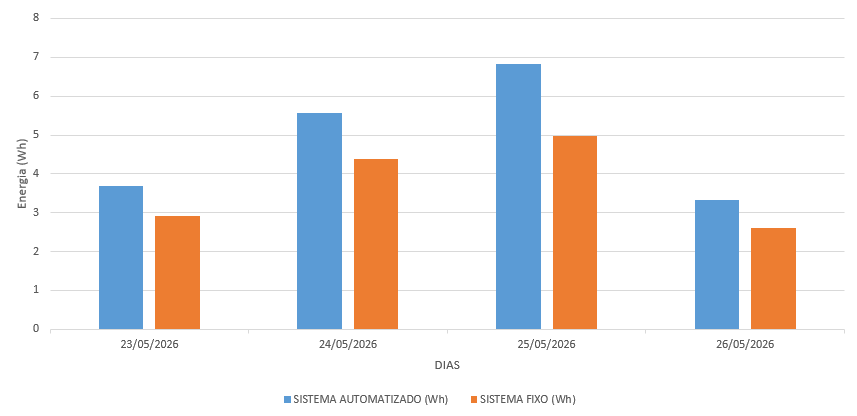
\includegraphics[width=0.85\textwidth]{Figuras/Energia_Acumulada.png}
    \caption{Energia acumulada diária dos sistemas fotovoltaicos automatizado e fixo.}
    \label{fig:energia_Acumulada}
    \fonte{Autor (2026).}
\end{figure}

Os valores numéricos da energia acumulada diária obtidos para cada sistema são apresentados na Tabela~\ref{tab:energia_diaria}.

\begin{table}[H]
\centering
\caption{Energia acumulada diária dos sistemas avaliados.}
\label{tab:energia_diaria}
\begin{tabular}{ccc}
\hline
Dia & Sistema automatizado (Wh) & Sistema fixo (Wh)\\
\hline
23/05/2026 & 3,70 & 2,92\\
24/05/2026 & 5,56 & 4,39\\
25/05/2026 & 6,82 & 4,98\\
26/05/2026 & 3,34 & 2,60\\
\hline
\end{tabular}
\fonte{Autor (2026).}
\end{table}

Para quantificar o desempenho do sistema automatizado em relação ao sistema com painel fixo, foi calculado o ganho energético percentual por meio da Equação~\ref{eq:ganho_energia}.

\begin{equation}
G(\%)=
\frac{E_{auto}-E_{fixo}}
{E_{fixo}}
\times100
\label{eq:ganho_energia}
\end{equation}

em que $E_{auto}$ representa a energia produzida pelo sistema automatizado e $E_{fixo}$ corresponde à energia produzida pelo sistema com painel fixo.

A análise da Figura~\ref{fig:energia_Acumulada} e da Tabela~\ref{tab:energia_diaria} mostra que o sistema automatizado apresentou maior produção de energia em todos os dias avaliados. O maior valor foi registrado em 25/05/2026, quando o sistema automatizado produziu aproximadamente 6,82 Wh, enquanto o sistema com painel fixo produziu 4,98 Wh. Nesse mesmo dia foi observado o maior ganho energético entre as duas configurações, de aproximadamente 36,95\%, indicando que, nas condições ambientais verificadas durante esse ensaio, o sistema automatizado obteve maior aproveitamento da irradiância incidente.

Os ganhos energéticos obtidos foram de 26,71\%, 26,65\%, 36,95\% e 28,46\% para os dias 23, 24, 25 e 26 de maio de 2026, respectivamente. Considerando todo o período experimental, o sistema automatizado acumulou aproximadamente 19,42 Wh, enquanto o sistema com painel fixo produziu cerca de 14,89 Wh, resultando em um ganho energético médio de aproximadamente 29,69\%.

Cabe destacar que os ganhos energéticos apresentados referem-se exclusivamente à energia elétrica produzida pelos módulos fotovoltaicos durante os ensaios experimentais. Não foi realizado o balanço energético considerando o consumo dos componentes utilizados no sistema automatizado, como o servomotor, o microcontrolador Arduino Uno, o display LCD, o módulo RTC, o cartão microSD e os sensores. Dessa forma, os valores obtidos representam o ganho da energia gerada pelo reposicionamento automático do painel, não correspondendo ao ganho líquido de energia do sistema completo. A avaliação do consumo energético do sistema de automação e sua influência sobre o ganho energético global constituem uma oportunidade para trabalhos futuros.

Esses resultados confirmam que o reposicionamento automático do painel proporcionou aumento consistente da energia produzida ao longo de todo o período experimental. Apesar das variações observadas entre os dias de coleta, decorrentes principalmente das condições ambientais, o sistema automatizado apresentou desempenho superior em todos os ensaios realizados, evidenciando a eficácia da estratégia de orientação adotada para maximizar o aproveitamento da radiação solar.